\newpage
\clearpage

% 3. Ejercicio 18:
\section{Ejercicio 23}

% 3.1. Enunciado:
\subsection{Enunciado}
\noindent Halla la distancia entre las rectas $r_1) \begin{cases}
	x = 2 + 2t \\
	y = -1 - t \\
	z = 3 + 3t
\end{cases} \ t \in \mathbb{R}$ y $r_2$ determinada por los puntos $P(1, 0, 2)$ y $Q(-2, 2, 6)$.


% 3.2. Solución analítica:
\newpage
\subsection{Solución analítica}

% Valores iniciales:
\subsubsection*{Valores iniciales:}

\begin{multicols}{2}
	\noindent En $r_1)$: \\
	\indent $\boxed{P_1(2, -1, 3)}$ \\
	\indent $\boxed{\vec{u}=(2, -1, 3)}$

	\columnbreak
	\noindent En $r_2)$: \\
	\indent $\boxed{P_2(1, 0, 2)}$

	\indent $\vec{v}  =\overrightarrow{PQ}     \\
		\indent \vec{v}  = (-2, 2, 6) - (1, 0, 2) \\
		\indent \vec{v}  =(-2-1, \ 2-0, \ 6-2)    \\
		\indent \boxed{\vec{v}  =(-3,2,4)}$
\end{multicols}

\noindent $\overrightarrow{P_1P_2} = (1, 0, 2) - (2, -1, 3)$

\noindent $\overrightarrow{P_1P_2} = [1 - 2, \ 0 - (-1), \ 2 - 3]$

\noindent $\boxed{\overrightarrow{P_1P_2} = (-1, 1, -1)}$
\vspace{1cm}

\noindent \textbf{Verificación de coplanaridad entre $r_1$ y $r_2$}:

\noindent Para verificar si las rectas son coplanares o alabeadas calculamos el producto mixto $\overrightarrow{P_1P_2} \cdot (\vec{u} \times \vec{v})$:
\begin{align*}
	\vec{u} \times \vec{v} & = (2, -1, 3) \times (-3, 2, 4)                                                          \\
	\vec{u} \times \vec{v} & = \begin{vmatrix}
		                           i  & j  & k \\
		                           2  & -1 & 3 \\
		                           -3 & 2  & 4 \\
	                           \end{vmatrix}                                                                        \\
	\vec{u} \times \vec{v} & = \vec{i} [(-1)(4) - (3)(2)] + \vec{j} [(3)(-3) - (2)(4)] + \vec{k} [(2)(2) - (-1)(-3)] \\
	\vec{u} \times \vec{v} & = \vec{i} (-4 - 6) + \vec{j} (-9 - 8) + \vec{k} (4 - 3)                                 \\
	\vec{u} \times \vec{v} & = \vec{i} (-10) + \vec{j} (-17) + \vec{k} (1)                                           \\
	\vec{u} \times \vec{v} & = (-10, \ -17, \ 1)
\end{align*}
\begin{align*}
	\overrightarrow{P_1P_2} \cdot (\vec{u} \times \vec{v}) & = (-1, 1, -1) \cdot (-10, -17, 1)      \\
	\overrightarrow{P_1P_2} \cdot (\vec{u} \times \vec{v}) & = [(-1)(-10)] + [(1)(-17)] + [(-1)(1)] \\
	\overrightarrow{P_1P_2} \cdot (\vec{u} \times \vec{v}) & = (10 - 17 -1)                         \\
	\overrightarrow{P_1P_2} \cdot (\vec{u} \times \vec{v}) & = (10 - 18)                            \\
	\overrightarrow{P_1P_2} \cdot (\vec{u} \times \vec{v}) & = \boxed{- 8}
\end{align*}

\noindent $\therefore$ \ podemos determinar que $r_1$ y $r_2$ son rectas \textbf{alabeadas}.








% 3.2.1. Cálculo de la distancia entre rectas:
\newpage
\subsubsection{\texorpdfstring{Distancia entre $r_1$ y $r_2$:}{}}
\noindent Para determinar la distancia entre $r_1$ y $r_2$ hacemos uso de la siguiente expresión:

\begin{center}
	$\boxed{\delta(r_1;r_2)
			= \left |Proy_{\vec{u} \times \vec{v}} \ \overrightarrow{P_1P_2} \right|
			= \left|\overrightarrow{P_1P_2} \cdot \dfrac{\vec{u} \times \vec{v}}{|\vec{u} \times \vec{v}|} \right|}$
\end{center}

\noindent Realizamos los cálculos:
\begin{align*}
	\delta(r_1;r_2) & = \left|\overrightarrow{P_1P_2} \cdot \dfrac{\vec{u} \times \vec{v}}{|\vec{u} \times \vec{v}|} \right| \\
	\delta(r_1;r_2) & = \left|\dfrac{\overrightarrow{P_1P_2} \cdot \vec{u} \times \vec{v}}{|\vec{u} \times \vec{v}|} \right| \\
	\delta(r_1;r_2) & = \left|\dfrac{-8}{(-10, -17, 1)} \right|                                                              \\
	\delta(r_1;r_2) & = \left|\dfrac{-8}{\sqrt{(-10)^2 + (-17)^2 +  (1)^2}} \right|                                          \\
	\delta(r_1;r_2) & = \left|\dfrac{-8}{\sqrt{100 + 289 +  1}} \right|                                                      \\
	\delta(r_1;r_2) & = \left|\dfrac{-4}{195}\sqrt{390} \right|                                                              \\
	\delta(r_1;r_2) & = \dfrac{4}{195}\sqrt{390}                                                                             \\
	\delta(r_1;r_2) & \approx 0.405                                                                                          \\
\end{align*}
$\therefore$ \ La distancia entre las rectas $r_1$ y $r_2$ es \fcolorbox{black}{yellow}{$\approx 0.405$}.

\newpage
\noindent \textbf{Gráfica 23}:
\begin{center}
	\href{https://www.geogebra.org/3d/ghqqu7e7}{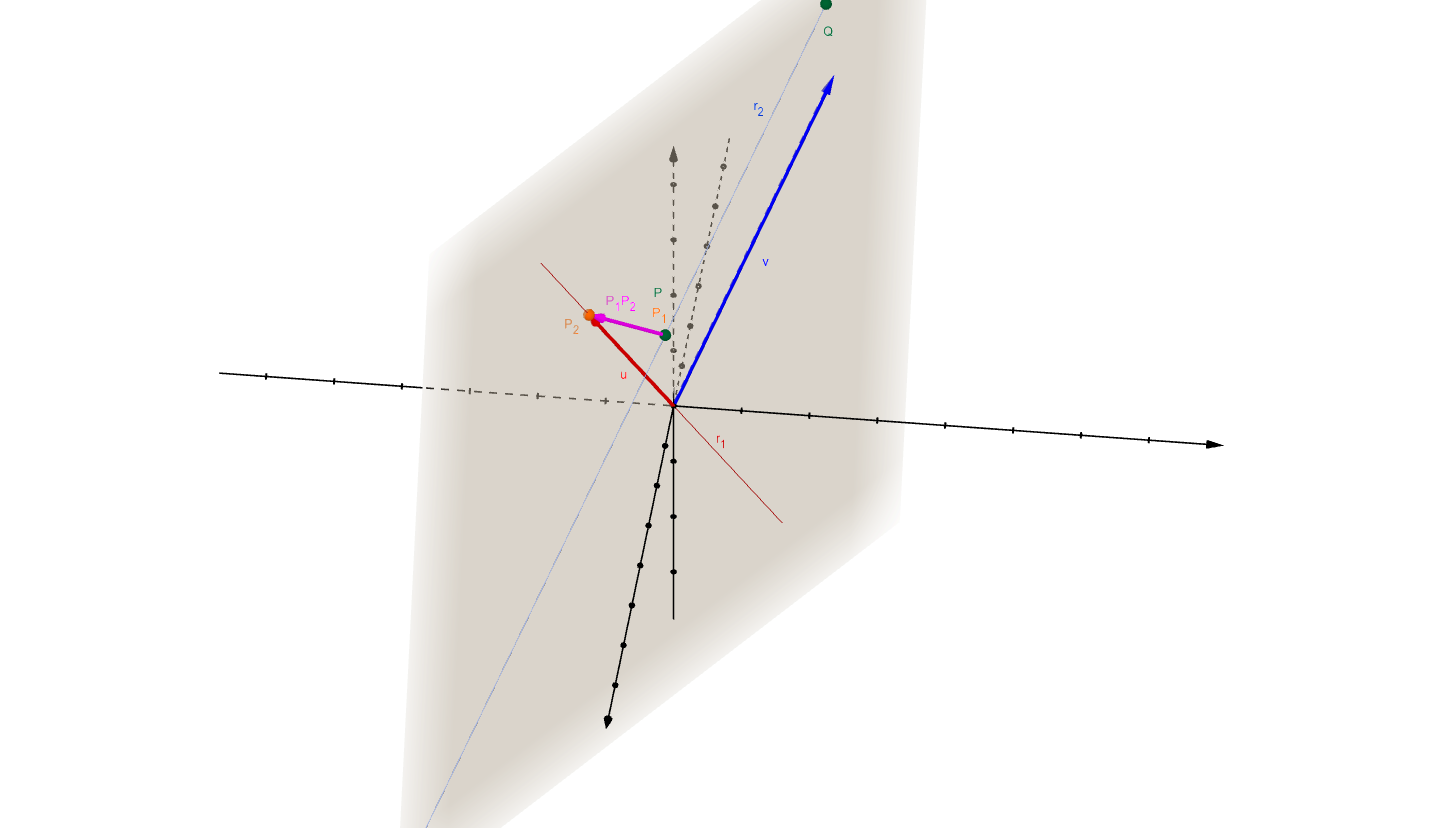
\includegraphics[width=15cm, scale=1]{TP-MATEMATICA-EJ23.png}}
\end{center}


%\noindent Con la situación y los valores iniciales anteriormente mencionados procedemos a hallar la distancia del punto $B$ al plano $\alpha$, para ello hallamos el módulo de la proyección $\vec{p}$:
\begin{center}
	$|\vec{p}|  =\cfrac{|\vec{b} \cdot \vec{n}|}{|\vec{n}|} \hspace*{1cm} \vec{b}=(2, 1, -1) \hspace*{1cm} \vec{n}=(3, 2, -5)$
\end{center}
\begin{multicols}{2}
	\noindent Hallamos el producto escalar entre $\vec{b} \cdot \vec{n}$:
	\begin{align*}
		\vec{b} \cdot \vec{n} & = (2) \cdot (3) + (1) \cdot (2) + (-1) \cdot (-5) \\
		\vec{b} \cdot \vec{n} & = 6 + 2 + 5                                       \\
		\vec{b} \cdot \vec{n} & = \boxed{13}
		\columnbreak
	\end{align*}
	\noindent Hallamos el módulo de $\vec{n}$:
	\begin{align*}
		|\vec{n}| & = \sqrt{(3)^2 + (2)^2 + (-5)^2} \\
		|\vec{n}| & = \sqrt{9 + 4 + 25}             \\
		|\vec{n}| & = \boxed{\sqrt{38}}
	\end{align*}
\end{multicols}
\noindent Hallamos el módulo de la proyección de $\vec{b}$ sobre $\vec{n}$:

$|\vec{p}| =\cfrac{13}{\sqrt{38}} \implies \cfrac{13}{38}\sqrt{38}$

\noindent $\therefore$ \ La distancia del punto $B$ al plano $\alpha$ es \ \fcolorbox{black}{yellow}{$\cfrac{13}{38}\sqrt{38}$}  $\approx 2,109$

% 2.2.2. Coordenadas de B':
%\newpage
%\subsubsection{\texorpdfstring{Coordenadas del punto $B'$ que pertenece a $\alpha$ y cuya distancia a $B$ es igual que la distancia de $B$ a $\alpha$:}{}}
%\noindent Para hallar el punto $B' \in \alpha$ y cuya distancia a $B$ es igual a la distancia de $B$ a $\alpha$ podemos hacer uso del vector proyección $\vec{p}$ antes mencionado para luego restarlo del vector $\vec{b}$, lo que nos da como resultado un vector $\vec{b'}$ cuyo sentido (punta flecha) coincidirá con el punto $B' \in \alpha$:
\begin{center}
	$\boxed{\vec{p} = \cfrac{\vec{b} \cdot \vec{n}}{|\vec{n}|^2} \cdot \vec{n}} \hspace*{1cm}
		\vec{n}=(3, 2, -5)  \hspace*{1cm}
		\vec{b}=(2, 1, -1) \hspace*{1cm}
		\vec{b} \cdot \vec{n}  = 13 \hspace*{1cm}
		|\vec{n}|  = \sqrt{38}$
\end{center}
\begin{multicols}{2}
	\noindent Calculamos $\vec{p}$:
	\begin{align*}
		\vec{p} & = \cfrac{\vec{b} \cdot \vec{n}}{|\vec{n}|^2} \cdot \vec{n}       \\
		\vec{p} & = \cfrac{13}{(\sqrt{38})^2} \cdot (3, 2, -5)                     \\
		\vec{p} & = \cfrac{13}{38} \cdot (3, 2, -5)                                \\
		\vec{p} & = \left( \cfrac{39}{38}, \cfrac{26}{38}, -\cfrac{65}{38} \right) \\
	\end{align*}
	\noindent Calculamos $\vec{b'}$:
	\begin{align*}
		\vec{b'} & = \vec{b} - \vec{p}                                                           \\
		\vec{b'} & = (2, 1, -1) - \left( \cfrac{39}{38}, \cfrac{26}{38}, -\cfrac{65}{38} \right) \\
		\vec{b'} & = \left( 2 - \cfrac{39}{38}, 1 - \cfrac{26}{38}, -1 + \cfrac{65}{38} \right)  \\
		\vec{b'} & = \left( \cfrac{37}{38}, \cfrac{12}{38}, \cfrac{27}{38} \right)
	\end{align*}
\end{multicols}

\noindent $\therefore$ \ Las coordenadas del punto $B'$ que está contenido en $\alpha$ y cuya distancia a $B$ es igual a la distancia de $B$ a $\alpha$ es:

\fcolorbox{black}{yellow}{$B'\left( \cfrac{37}{38}, \cfrac{12}{38}, \cfrac{27}{38} \right)$}
\ $\approx \ (0.974; \ 0.316;\ 0.711)$

\newpage
\noindent \textbf{Gráfica 18-a,b}:
\begin{center}
	\href{https://www.geogebra.org/3d/wrk3eabw}{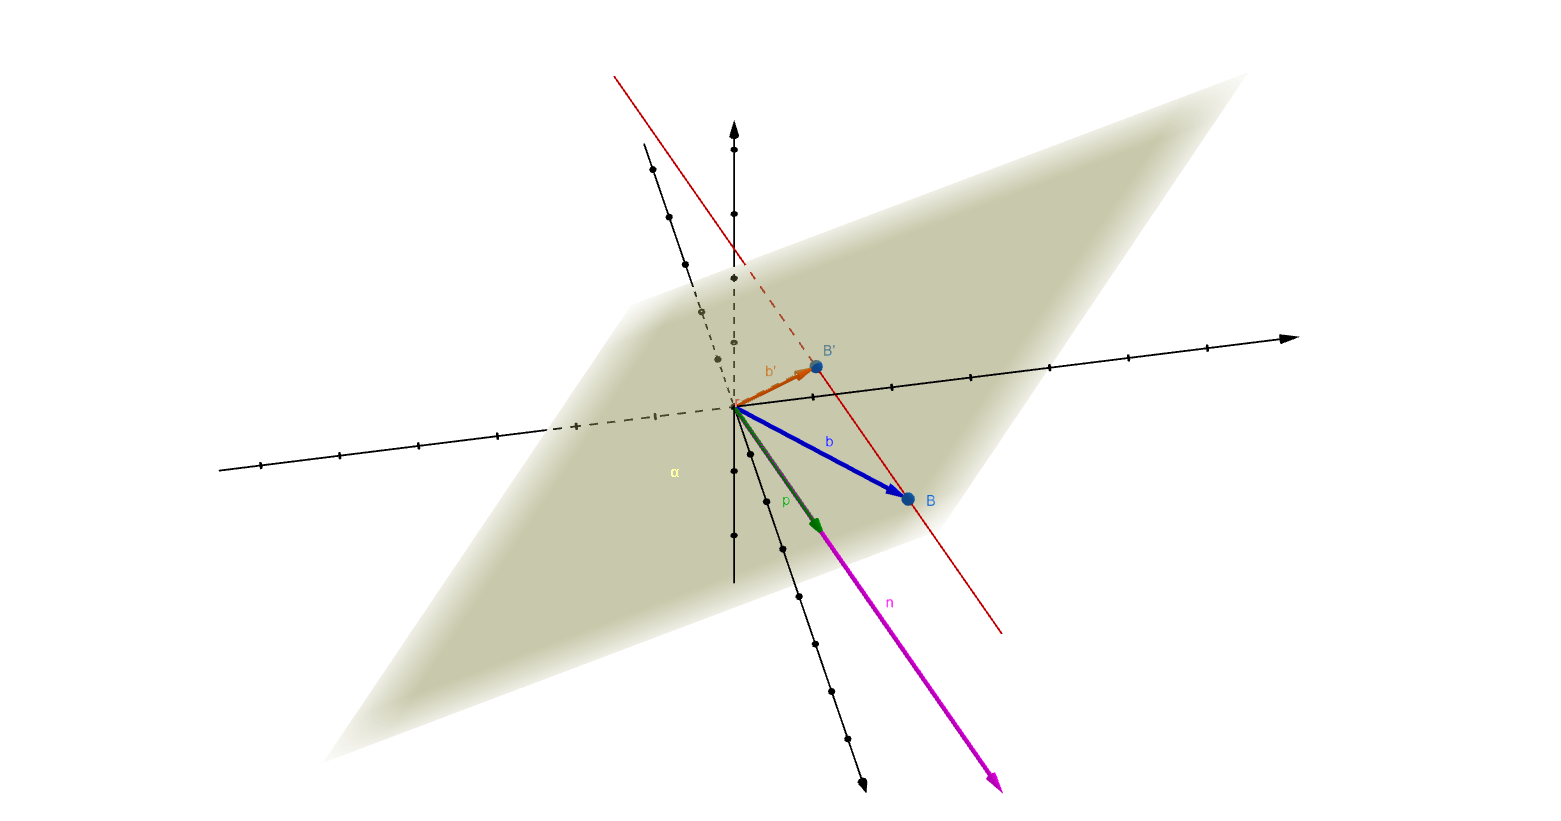
\includegraphics[width=15cm, scale=1]{TP-MATEMATICA-EJ18AB.png}}
\end{center}



